\documentclass[12pt,a4paper,oneside]{book} 
\usepackage[utf8]{inputenc}
\usepackage[spanish]{babel}
\usepackage{amsmath}
\usepackage{array}
\usepackage{amsfonts}
\usepackage{amssymb}
\usepackage{abstract} % Allows abstract customization
\renewcommand{\abstractnamefont}{\normalfont\bfseries} % Set the "Abstract" text to bold
\renewcommand{\abstracttextfont}{\normalfont\small\itshape} % Set the abstract itself to small italic text


\usepackage{amssymb, amsmath}
\usepackage{graphicx}
\usepackage[left=2.54cm,right=2.54cm,top=2.54cm,bottom=2.54cm]{geometry}

\begin{document}
	
	\thispagestyle{empty} 
	
	\begin{center} 
		\LARGE{UNIVERSIDAD PRIVADA DE TACNA} \\[0.5cm] 
		\Large{FACULTAD DE INGENIERÍA DE SISTEMAS}\\[0.5cm] 
		\large{ ESCUELA PROFESIONAL DE INGENIERÍA SISTEMAS} 
	\end{center}
	
	\begin{figure}[htb]
		\centering 
\includegraphics[width=6cm, height=7cm]{img/uptlogo.jpg}
	\end{figure}
	
	\begin{center} 
			\LARGE{\bf PROYECTO TRABAJO FINAL \newline UNIDAD III }\\ \vspace{.25cm}
		
	\end{center}

	\begin{center} 
		
		\textbf {CURSO}\\ 
		\large CALIDAD Y PRUEBAS DE SOFTWARE Sec. A \\
		
		\textbf {DOCENTE}\\
		\large Mag. Patrick Cuadros Quiroga\\
	
		\textbf {INTEGRANTES}\\
		\large Tarqui Montalico, Risther Jaime - 2017057857 \\
		\large Limache Victorio, V\'ictor Piero - 2017057857 \\
		\large Catari Cabrera Yober Nain - 2017059289 \\
		\large Liendo Velasquez, Joaqu\'in - 2017057857 \\
		\large Callata Flores, Rafael - 2017057857 \\
		
	\end{center}

	
	
	\begin{center} 
		\Large \textsc{Tacna - Perú} \\
		\Large \textsc{2020 } 
	\end{center}

	\newpage
	
	%%INICIO abstract
	\begin{abstract}

		Con el auge de las aplicaciones web y basadas en la nube, han surgido numerosas herramientas de software que nos permiten gestionar diversas tareas. En el área de ingeniería de software y en particular testing de software (Software Testing), existen nuevas herramientas para registrar información y presentar informes de estado en las diferentes fases del ciclo de vida, de acuerdo con las metodologías de desarrollo de software utilizadas. También contamos con nuevas herramientas para automatizar Pruebas.\\
		
		\begin{center}
			
			\textbf{Abstract}
		\end{center}
	
		With the rise of web and cloud-based applications, numerous software tools have emerged that allow us to manage various tasks. In the area of software engineering and in particular software testing (Software Testing), there are new tools to record information and present status reports in the different phases of the life cycle, according to the software development methodologies used. We also have new tools to automate Tests.\\
		
	\end{abstract}
	%%FIN abstract
	
	\newpage
	
	\begin{center} 
		\LARGE{\bf PROYECTO TRABAJO FINAL \newline UNIDAD III }\\ \vspace{.25cm}
	\end{center}
	
	\begin{enumerate}
		\item \textbf{INTRODUCCION}
			Es fundamental para cualquier proyecto, salvo que sea muy pequeño, contar con alguna herramienta de gestión de pruebas. Hay herramientas que van por separado y otras que integran con herramientas complementarias, por ejemplo, con las de «bug tracking».\\
			A continuación, en este trabajo encargado, veremos una comparativa entre dos herramientas de pruebas mas conocidas hoy en día como lo son: AWS CodePipeline y Azure DevOps.\\
			
		\item \textbf{TITULO}
			Herramientas de Gestión de Pruebas. \\
		\item \textbf{AUTORES}
			\begin{itemize}
				 \item Tarqui Montalico, Risther Jaime 
				 \item Limache Victorio, V\'ictor Piero 
				 \item Catari Cabrera Yober Nain 
				 \item Liendo Velasquez, Joaqu\'in 
				 \item Callata Flores, Rafael 
			\end{itemize}
		\item \textbf{DESARROLLO}
			\begin{itemize}
				\item \textbf{¿QUÉ SON LAS HERRAMIENTAS DE GESTIÓN DE PRUEBAS?}
					Es la herramienta que proporciona soporte a la gestión de pruebas y control de parte del proceso de pruebas. A menudo tiene varias capacidades, tales como gestionar los productos de soporte de pruebas, planificación de pruebas, registro de resultados, seguimiento del proceso, gestión de incidencias y generación de informes de las pruebas.\\
				\item \textbf{¿QUÉ ES AWS CODEPIPELINE?}
					Es un servicio de Amazon Web Services que nos ayuda a automatizar los procesos de lanzamiento para obtener actualizaciones rápidas y confiables. AWS Codepipeline compila, prueba e implementa tu código cada vez que hay un cambio, en función a los modelos de proceso de los releases que hagas.\\
					
			\newpage			
						\begin{center}
							\begin{figure}[htb]
								\centering 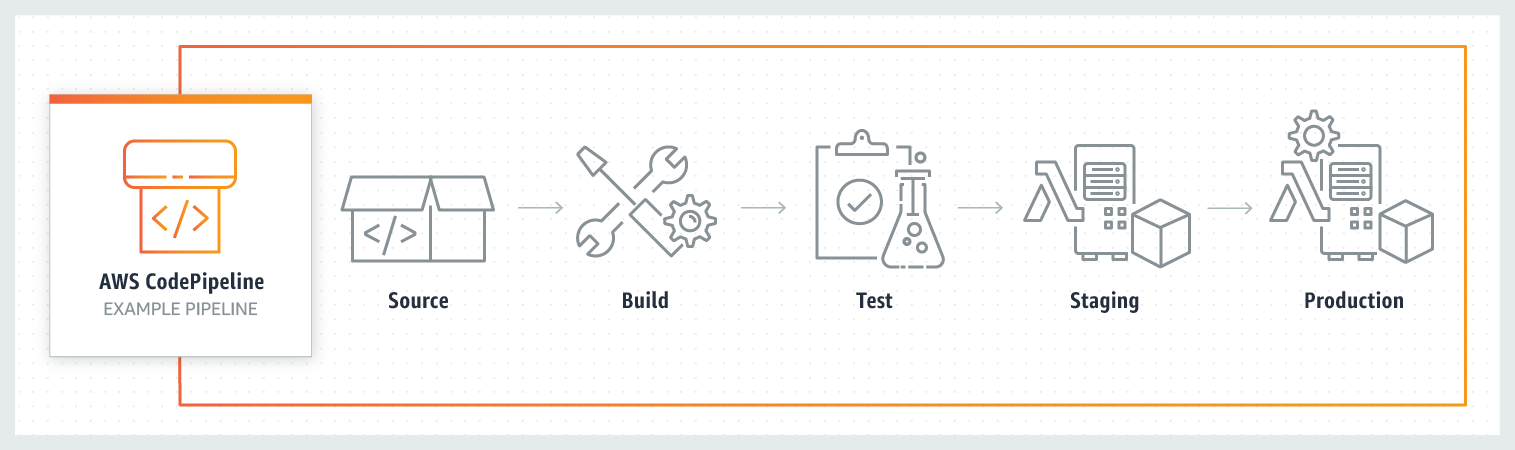
\includegraphics[width=10cm, height=3cm]{img/code.png}
							\end{figure}
						\end{center}
						
					
				\item \textbf{¿QUÉ ES AZURE DEVOPS?}
					Es una plataforma de SaaS (software como servicio) de Microsoft que nos proporciona una cadena de herramientas DevOps de punto a punto para desarrollar e implementar software. También proporciona alojamiento Git privado ilimitado, compilación en la nube para la integración continua, planificación ágil y administración de versiones para la entrega continua a la nube y en las instalaciones. Incluye amplio soporte IDE.\\
					\begin{center}
						\begin{figure}[htb]
							\centering 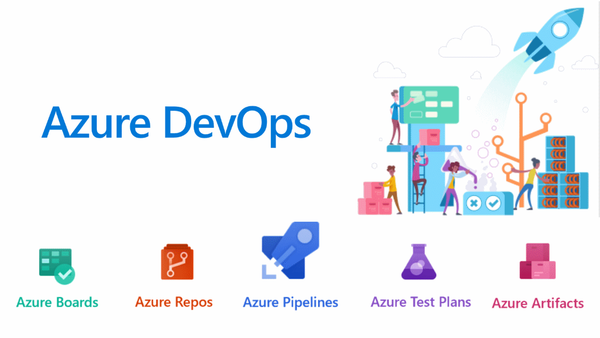
\includegraphics[width=10cm, height=5cm]{img/azure.png}
						\end{figure}
					\end{center}
						
				\item \textbf{COMPARATIVA ENTRE AMBOS: VENTAJAS}
					\begin{center}
						\begin{figure}[htb]
							\centering 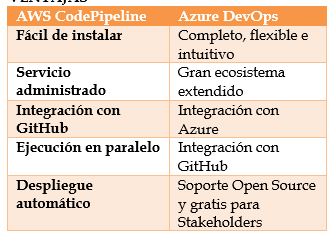
\includegraphics[width=8cm, height=5cm]{img/comparativa1.png}
						\end{figure}
					\end{center}
		 \newpage
				\item \textbf{COMPARATIVA ENTRE AMBOS: DESVENTAJAS}
					\begin{center}
						\begin{figure}[htb]
							\centering 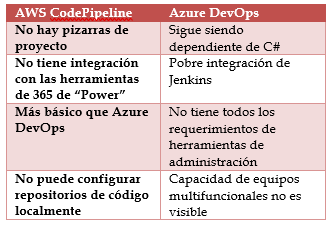
\includegraphics[width=8cm, height=5cm]{img/comparativa2.png}
						\end{figure}
					\end{center}
					
				\item \textbf{COMPAÑIAS QUE USAN ESTAS HERRAMIENTAS:}
					\begin{center}
						\begin{figure}[htb]
							\centering \includegraphics[width=8cm, height=5cm]{img/compañias.png}
						\end{figure}
					\end{center}
				\item \textbf{HERRAMIENTAS QUE PUEDEN SER INTEGRADAS:}
					\begin{center}
						\begin{figure}[htb]
							\centering 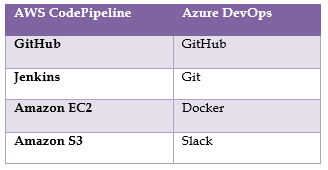
\includegraphics[width=10cm, height=5cm]{img/herramientas.png}
						\end{figure}
					\end{center}
					
				\item \textbf{ALGUNAS BUENAS ALTERNATIVAS A AMBOS:}
						\begin{enumerate}
							\item AWS CodeDeploy
							\item Jenkins
							\item AWS CodeBuild
							\item TeamCity
							\item Bamboo
						\end{enumerate}
			\end{itemize}
		\item \textbf{CONCLUSIONES}
				\begin{enumerate}
					\item CodePipeLine
						\begin{itemize}
							\item CodePipeline es una herramienta de entrega continua e integración continua muy flexible.
							\item Facilita un poco la implementación en el entorno de AWS. Hay una gran disponibilidad de datos no estructurados.
							\item Se usa bastante para gestionar la CI/CD (Integración continua e integración delivery)
							
						\end{itemize}
					\item Azure DevOps
						\begin{itemize}
							\item Es muy fácil de configurar y usar si tiene alguna experiencia con procesos ágiles. 
							\item Las barreras de entrada iniciales son extremadamente bajas, ya que los primeros 5 usuarios pueden aprovechar la herramienta de forma gratuita. Encontré la característica / funcionalidad general más fácil de usar y más accesible que herramientas similares. 
							\item Si ya es un usuario de git, esto se integra directamente con los repositorios de git, lo que facilita la transición. 
							\item La herramienta también está integrada con muchos otros productos de Microsoft, por lo que si tiene una tienda centrada en Microsoft, puede aprovechar el ecosistema más amplio.
							
							
						\end{itemize}
				\end{enumerate}
				
		
		\item \textbf{RECOMENDACIONES}
			Aquí una serie de aspectos a tener en cuenta al momento de elegir una herramienta para la gestión de prueba.
			
			\begin{itemize}
				\item La categoría de defectos
				\item El lenguaje de programación y entorno de desarrollo
				\item El proceso de configuración y gestión de datos de prueba
				\item El control de versiones y CI (Integración Contínua)
				\item Los reportes
				\item Las plataformas compatibles y etiquetado
				
			\end{itemize}
			
		\item \textbf{BIBLIOGRAFIA}
			\begin{itemize}
				
			\item https://stackshare.io/stackups/aws-codepipeline-vs-azure-devops\#:~:text=AWS\%20CodePipeline\%20belongs\%20to\%20\%22Continuous,Workflow\%20Modeling
			
			\item https://www.trustradius.com/products/aws-codepipeline/reviews
			
			\item https://www.trustradius.com/compare-products/aws-codepipeline-vs-azure-devops
			
			\item https://www.infoworld.com/article/3271126/what-is-cicd-continuous-integration-and-continuous-delivery-explained.html
			 
			\end{itemize}
		
	\end{enumerate}
	
	
	

\end{document}
